\chapter{Graphs}
\section{The Basics}

% 1.1 Recall (Text Block)
\topic{Recall}

\begin{enumerate}
    \item A \textbf{set} is merely an accumulation of objects. These objects are called \textbf{elements} of the set. If an object $x$ is an element of $S$, we write $x \in S$. The set of all elements with a certain property $P$ is denoted via $\{x \mid x \text{ has property } P\}$.
    
    \item An \textbf{$n$-ary relation} $R$ on a set $A$ is a subset of the power set of $A^n$, i.e., $R \subseteq \mathcal{P}(A^n)$. If $n=2$, we call the relation \textbf{binary}.
    
    A binary relation $R$ on a set $A$ is called:
    \begin{itemize}
        \item[(i)] \textbf{symmetric} if $R(a,b)$ implies $R(b,a)$ for all $a,b \in A$.
        \item[(ii)] \textbf{asymmetric} if $R(a,b)$ implies $\neg R(b,a)$ for all $a,b \in A$.
        \item[(iii)] \textbf{antisymmetric} if $R(a,b) \land R(b,a)$ implies $a=b$ for all $a,b \in A$.
        \item[(iv)] \textbf{reflexive} if $R(a,a)$ for all $a \in A$.
        \item[(v)] \textbf{irreflexive} if $\neg R(a,a)$ for all $a \in A$.
        \item[(vi)] \textbf{transitive} if $R(a,b) \land R(b,c)$ implies $R(a,c)$ for all $a,b,c \in A$.
    \end{itemize}
\end{enumerate}

% 1.2 Definition (Red Box)
\begin{definition}
A \textbf{graph} $G=(V,E)$ is a pair of sets $V$ and $E$ s.t. $E$ consists of subsets of $V$ of size two. $V$ is called the set of \textbf{vertices} and $E$ the set of \textbf{edges}. A graph $G$ is called \textbf{finite} if $V$ is a finite set. The \textbf{order} $|G|$ of a graph $G=(V,E)$ is the cardinality of its vertex set, so $|G|=|V|$. The \textbf{size} $\|G\|$ of $G$ is the cardinality of its edge set, $\|G\|=|E|$.
\end{definition}

% 1.3 Visualisation (Text Block)
\topic{Visualisation}

Let $G=(V,E)$ be a graph. We visualise vertices $u,v \dots \in V$ by dots and edges $e=\{u,v\} \in E$ by the diagram:

\begin{center}
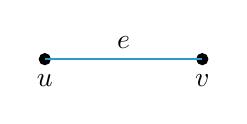
\begin{tikzpicture}
    \filldraw (0,0) circle (2pt) node[below=2pt] {$u$};
    \filldraw (2,0) circle (2pt) node[below=2pt] {$v$};
    \draw[cyan!80!black, thick] (0,0) -- (2,0) node[midway, above, black] {$e$};
\end{tikzpicture}
\end{center}

% 1.4 Example (Text Block)
\begin{example}[Bowtie Graph]
Let $G=(V,E)$ be the graph with $V=\{a,b,c,d,e\}$ and
\[ E = \{\{a,b\}, \{a,c\}, \{a,d\}, \{a,e\}, \{b,c\}, \{d,e\}\}. \]
The graph $G$ has order 5 and size 6. It can be visualized via:
\begin{center}
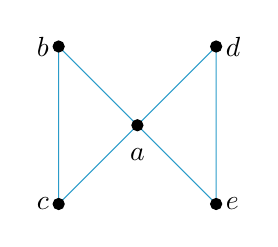
\begin{tikzpicture}
    \coordinate (a) at (0,0);
    \coordinate (b) at (-1,1);
    \coordinate (c) at (-1,-1);
    \coordinate (d) at (1,1);
    \coordinate (e) at (1,-1);

    \draw[cyan!80!black] (b) -- (a) -- (c) -- (b);
    \draw[cyan!80!black] (d) -- (a) -- (e) -- (d);

    \filldraw (a) circle (2pt) node[below=5pt] {$a$};
    \filldraw (b) circle (2pt) node[left] {$b$};
    \filldraw (c) circle (2pt) node[left] {$c$};
    \filldraw (d) circle (2pt) node[right] {$d$};
    \filldraw (e) circle (2pt) node[right] {$e$};
\end{tikzpicture}
\end{center}
This visualisation motivates its name: \textbf{bowtie graph}.
\end{example}

% 1.5 Notation
\topic{Notation}

\begin{enumerate}
    \item For a graph $G=(V,E)$ we may denote its vertex set by $V(G)$ or $V_G$ for clarity.
    \item Similarly, we often denote $E$ by $E(G)$ or $E_G$.
    \item We denote an edge $\{u,v\}$ simply by $uv$.
    \item Edges are often called $e, e_1, e_2, f \dots$, while vertices are called $u, v, x, y, \dots$.
\end{enumerate}

% 1.6 Definition
\begin{definition}
Let $G=(V,E)$ be a graph.
\begin{enumerate}
    \item If $uv \in E$ is an edge, then we say that $u$ and $v$ are \textbf{adjacent} or \textbf{neighbours}. If $uv \notin E$, we call $u$ and $v$ \textbf{nonadjacent}.
    \item If $e=uv \in E$, we say that $u$ and $v$ are the \textbf{end vertices} of $e$ or that they are \textbf{incident} with $e$.
    \item The \textbf{neighborhood} $N(v)$ of a vertex $v \in V$ is the set of all vertices adjacent to $v$, i.e., $N(v) = \{u \in V \mid uv \in E\}$. The \textbf{closed neighborhood} $N[v]$ of $v$ is $N[v] := N(v) \cup \{v\}$.
    \item The \textbf{neighborhood} $N(S)$ of a set of vertices is defined as $N(S) := \bigcup_{v \in S} N(v)$. Similarly, the \textbf{closed neighborhood} $N[S]$ is set to be $N[S] := N(S) \cup S (= \bigcup_{v \in S} N[v])$.
    \item The \textbf{degree} $\deg(v)$ of $v \in V$ is the number of edges incident with $v$, i.e., $\deg(v) := |\{e \in E \mid v \in e\}| = |N(v)|$.
    \item The \textbf{maximum degree} $\Delta(G)$ of $G$ is defined as
    \[ \Delta(G) := \max \{ \deg(v) \mid v \in V \}. \]
    Similarly, $\delta(G) := \min \{ \deg(v) \mid v \in V \}$ is the \textbf{minimum degree} of $G$.
    \item The \textbf{degree sequence} of a graph $G$ is the sequence containing all degrees of the vertices of $G$ (with repetition) in decreasing order.
\end{enumerate}
\end{definition}

% 1.7 Example
\begin{example}
Consider $G$ given by:
\begin{center}
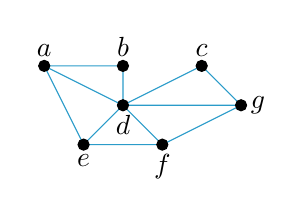
\begin{tikzpicture}
    \coordinate (a) at (0,1);
    \coordinate (b) at (1,1);
    \coordinate (c) at (2,1);
    \coordinate (d) at (1,0.5);
    \coordinate (e) at (0.5,0);
    \coordinate (f) at (1.5,0);
    \coordinate (g) at (2.5,0.5);

    \draw[cyan!80!black] (a) -- (d) -- (b) -- (a) -- (e) -- (d) -- (f) -- (e);
    \draw[cyan!80!black] (d) -- (g) -- (c) -- (d);
    \draw[cyan!80!black] (f) -- (g);

    \foreach \point in {a,b,c,d,e,f,g} \filldraw (\point) circle (2pt);
    \node[above] at (a) {$a$}; \node[above] at (b) {$b$}; \node[above] at (c) {$c$};
    \node[below] at (d) {$d$}; \node[below] at (e) {$e$}; \node[below] at (f) {$f$}; \node[right] at (g) {$g$};
\end{tikzpicture}
\end{center}
Then $\Delta(G)=5$, $\delta(G)=1$. $N(e)=\{a,d,f\}$, $N[b]=\{b,d\}$.
\end{example}

% 1.8 Example
\begin{example}
Consider $G$ given via the diagram:
\begin{center}
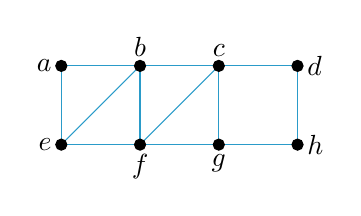
\begin{tikzpicture}
    \coordinate (a) at (0,1); \node[left] at (a) {$a$};
    \coordinate (b) at (1,1); \node[above] at (b) {$b$};
    \coordinate (c) at (2,1); \node[above] at (c) {$c$};
    \coordinate (d) at (3,1); \node[right] at (d) {$d$};
    
    \coordinate (e) at (0,0); \node[left] at (e) {$e$};
    \coordinate (f) at (1,0); \node[below] at (f) {$f$};
    \coordinate (g) at (2,0); \node[below] at (g) {$g$};
    \coordinate (h) at (3,0); \node[right] at (h) {$h$};
    
    \draw[cyan!80!black] (a)--(b)--(c)--(d);
    \draw[cyan!80!black] (e)--(f)--(g)--(h);
    \draw[cyan!80!black] (a)--(e); \draw[cyan!80!black] (b)--(f); \draw[cyan!80!black] (c)--(g); \draw[cyan!80!black] (d)--(h);
    \draw[cyan!80!black] (b)--(e); \draw[cyan!80!black] (c)--(f);
    
    \foreach \p in {a,b,c,d,e,f,g,h} \filldraw (\p) circle (2pt);
\end{tikzpicture}
\end{center}
$|G|=9$, size of $G$ is 9. Degree sequence $(3,3,3,2,2,2,2,1,0)$.
\end{example}

% 1.9 Remark
\begin{remark}
A graph can be considered as a set $V$ together with a binary relation $E$ on $V$ which is symmetric and irreflexive.
\end{remark}

% 1.10 Definition
\topic{Definition (Variants of Graphs)}

\begin{enumerate}
    \item If $G=(V,E)$ and we replace $E$ with a set of ordered pairs, then we call $G$ a \textbf{directed graph} or \textbf{digraph}.
    \item If $E$ is a multiset (iterations of the same elements are distinguished), then we call $G$ a \textbf{multigraph}.
    \item If we extend $E$ by allowing loops, we call $G$ a \textbf{pseudograph}.
    \item If we allow edges to be arbitrary sets of vertices instead of 2-elementary ones, we call $G$ a \textbf{hypergraph}.
\end{enumerate}

% 1.11 Setting
\topic{Setting}
In this lecture, unless otherwise stated, by a graph we mean a finite, simple graph with $|V| \ge 1$.

% 1.12 Definition
\begin{definition}
\begin{itemize}
    \item The \textbf{complete graph} $K_n$ for $n \ge 1$ is the graph consisting of $n$ vertices such that any two vertices are adjacent.
    \item The \textbf{empty graph} $E_n$ is the graph consisting of $n$ vertices and no edges.
\end{itemize}
\end{definition}

% 1.13 The Handshaking Lemma
\begin{theorem}[The Handshaking Lemma]
If $G=(V,E)$ is a graph, then
\[ \sum_{v \in V} \deg(v) = 2|E|. \]
\end{theorem}

\begin{proof}
We proceed by induction on $n := |E|$.
\textbf{n=0:} If $|E|=0$, then $\deg(v)=0$ for any $v \in V$, whence clearly $0 = \sum \deg(v) = 2|E| = 0$.

\textbf{n $\to$ n+1:} Assume $(*)$ holds for any $G'=(V',E')$ with $|E'|=n$ (I.H.) and consider $G=(V,E)$ with $|E|=n+1 (\ge 1)$ arbitrary. Let $e \in E$ arbitrary and consider $G'=(V, E \setminus \{e\})$. Then, if $e=uv$, we get $|E(G)| = |E(G')|+1$ and
\[ \deg_G(u) = \deg_{G'}(u) + 1 \quad \text{and} \quad \deg_G(v) = \deg_{G'}(v) + 1, \]
whence
\[ 2|E(G)| = 2|E(G')| + 2 \overset{\text{I.H.}}{=} \sum_{w \in V} \deg_{G'}(w) + 2 \]
\[ = \sum_{w \in V \setminus \{u,v\}} \deg_{G'}(w) + \deg_{G'}(u) + 1 + \deg_{G'}(v) + 1 \]
\[ = \sum_{w \in V} \deg_G(w), \text{ as desired.} \qedhere \]
\end{proof}

% 1.14 Corollary
\begin{corollary}
Any graph $G$ has an even number of vertices of odd degree.
\end{corollary}
\begin{proof}
Exercise.
\end{proof}

% 1.15 Corollary
\begin{corollary}
For any graph $G=(V,E)$ we have
\[ \delta(G) \le 2 \frac{|E|}{|V|} \le \Delta(G). \]
\end{corollary}
\begin{proof}
\[ |V| \cdot \delta(G) = \sum_{v \in V} \delta(G) \le \sum_{v \in V} \deg(v) \le \sum_{v \in V} \Delta(G) = |V|\Delta(G) \]
Using Theorem 1.13, $\sum \deg(v) = 2|E|$. Dividing by $|V|$ yields the result.
\end{proof}

% 1.16 Lemma
\begin{lemma}
If $|G| \ge 2$, then $G$ contains at least two vertices of the same degree.
\end{lemma}
\begin{proof}
If $G$ has two vertices of degree 0, then we are done. Otherwise, we may assume that $G$ has none. If $|V|=n$, and $v \in V$, then $1 \le \deg(v) \le n-1$. Note that this leaves us with $n-1$ choices of degrees for $n$ many different vertices. Hence, at least two vertices must have the same degree.
\end{proof}

% 1.17 Remark
\begin{remark}
The above line of thought is called the \textbf{pigeon hole principle}. If there are $n$ many pigeons wanting to fit into $n-1$ many holes, then at least two of them have to cuddle up in the same hole.
\end{remark}

% 1.18 Definition
\begin{definition}
\begin{enumerate}
    \item The \textbf{path} $P_n$ is the graph on $n$ vertices $v_1, \dots, v_n$ with the edge set $E(P_n) = \{v_i v_{i+1} \mid 1 \le i < n\}$.
    \item The \textbf{cycle} $C_n$ is the graph on $n$ vertices with edge set $E(C_n) = \{v_i v_{i+1} \mid 1 \le i < n\} \cup \{v_n v_1\}$.
    \item Let $G=(V,E)$ be an arbitrary graph. The \textbf{complement} $\overline{G}$ of $G$ is the graph $\overline{G}=(V, \overline{E})$, where $\overline{E} = \{uv \mid u,v \in V, uv \notin E\}$.
\end{enumerate}
\end{definition}

% 1.19 Definition
\begin{definition}
We call a graph $G$ \textbf{regular} if any of its vertices has the same degree. If this degree is $r$, we say that $G$ is \textbf{$r$-regular}.
\end{definition}

% 1.20 Remarks
\begin{remark}
\begin{enumerate}
    \item A graph $G$ is regular iff $\delta(G)=\Delta(G)$.
    \item $K_n$ is $(n-1)$-regular and $E_n$ is $0$-regular.
    \item An $r$-regular graph of order $n$ has $\frac{1}{2}nr$ many edges.
\end{enumerate}
\end{remark}

% 1.21 Example
\begin{example}
The graph below is 4-regular of order 6.
\begin{center}
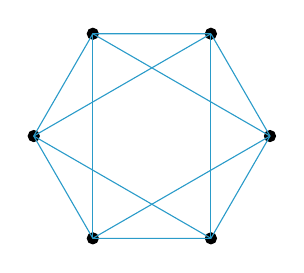
\begin{tikzpicture}
    % Octahedron graph projection
    \foreach \i in {1,...,6}
        \coordinate (v\i) at (60*\i:1.5);
    
    \foreach \i in {1,...,6} \filldraw (v\i) circle (2pt);
    
    \draw[cyan!80!black] (v1)--(v2)--(v3)--(v4)--(v5)--(v6)--(v1);
    \draw[cyan!80!black] (v1)--(v3); \draw[cyan!80!black] (v1)--(v5);
    \draw[cyan!80!black] (v2)--(v4); \draw[cyan!80!black] (v2)--(v6);
    \draw[cyan!80!black] (v3)--(v5); \draw[cyan!80!black] (v4)--(v6);
\end{tikzpicture}
\end{center}
\end{example}

\section{Subgraphs}

% 1.22 Definition
\begin{definition}
\begin{enumerate}
    \item A graph $H$ is called a \textbf{subgraph} of some graph $G$, written $H \subseteq G$, if $V(H) \subseteq V(G)$ and $E(H) \subseteq E(G)$. We also say $G$ \textbf{contains} $H$.
    \item If $H \subseteq G$, we say that $H$ is an \textbf{induced subgraph} of $G$, written $H \sqsubseteq G$, if $E(H) = \{uv \in E(G) \mid u,v \in V(H)\}$.
\end{enumerate}
\end{definition}

% 1.23 Remark
\begin{remark}
\begin{enumerate}
    \item $H \subseteq G$ is induced if for any two vertices in $H$ we have: If they are adjacent in $G$, then they are adjacent in $H$.
    \item Every induced subgraph is a subgraph but not vice versa.
    \item If $G$ is a graph and $S \subseteq V(G)$, then there is only one induced subgraph $H \sqsubseteq G$ with vertex set $S$, i.e. $V(H)=S$. We denote this graph by $\langle S \rangle$ and call it the subgraph of $G$ induced by $S$.
\end{enumerate}
\end{remark}

% 1.24 Example
\begin{example}
Consider $G$ given as... (Graph illustrations of subgraphs vs induced subgraphs).
\end{example}

\section{Walks in Graphs}

% 1.25 Definition
\begin{definition}
A $(v_0, v_k)$-\textbf{walk} in a graph is a sequence of vertices $(v_0, v_1, \dots, v_k)$ s.t. any two consecutive vertices $v_i$ and $v_{i+1}$ are adjacent. We call the edges $\{v_0v_1, v_1v_2, \dots, v_{k-1}v_k\}$ the \textbf{edges of the walk}. We say that the walk is \textbf{closed} if $v_0=v_k$. The \textbf{length} of a walk is the number of edges in it (counting repetition).
\end{definition}

% 1.26 Definition
\begin{definition}
We distinguish the following types of walks:
\begin{itemize}
    \item A \textbf{trail} is a walk whose edges are pairwise distinct.
    \item A \textbf{circuit} is a closed walk whose edges are pairwise distinct.
    \item A \textbf{path} is a walk whose vertices are distinct.
    \item A \textbf{cycle} is a closed walk $(v_0, \dots, v_k=v_0)$ with $k \ge 3$ and whose vertices $v_0, \dots, v_{k-1}$ are pairwise distinct.
\end{itemize}
\end{definition}

% 1.27 Example
\begin{example}
Consider $G$ via... (Examples of walks, trails, paths).
\end{example}

% 1.28 Lemma
\begin{lemma}
If $\delta(G) \ge 2$, then $G$ contains a cycle as a subgraph.
\end{lemma}
\begin{proof}
Let $P = (v_0, \dots, v_k)$ be a path in $G$ of maximal length. This exists, as $G$ is finite. Further, as $\delta(G) \ge 2$, we get $k \ge 2$. As $\deg(v_0) \ge \delta(G) \ge 2$, $v_0$ has at least two neighbors. One of them is $v_1$. Let us denote the other one by $u$. If $u \ne v_i$ for all $1 \le i \le k$, then $\tilde{P} = (u, v_0, v_1, \dots, v_k)$ is still a path and of greater length than $P$, contradicting our assumptions. Hence, $u=v_i$ for some $1 \le i \le k$. But then the sequence $(v_0, v_1, \dots, v_i=u, v_0)$ is the desired cycle subgraph of $G$.
\end{proof}

% 1.29 Corollary
\begin{corollary}[Contrapositive]
If $G$ does not contain any cycles, then $\delta(G) \le 1$.
\end{corollary}

% 1.30 Theorem
\begin{theorem}
Every $uv$-walk in a graph contains a $uv$-path.
\end{theorem}
\begin{proof}
We proceed by strong induction on the length $n \ge 1$ of the walk.
\textbf{I.B. n=1.} If the $uv$-walk is of length one, then it is exactly $(u,v)$, which is also a path.
\textbf{I.S.} Assume every $uv$-walk of length at most $n \ge 1$ contains a $uv$-path (I.H.). Assume there is a $uv$-walk $W=(u=w_0, w_1, \dots, w_n, w_{n+1}=v)$ of length $n+1$. If $W$ is already a path, we are done. Otherwise there are $i,j$ s.t. $0 \le i < j \le n+1$ and $w_i = w_j$. But then the walk $\tilde{W}$ which arises from $W$ by deleting the vertices $w_{i+1}, \dots, w_{j-1}, w_j$, i.e. $\tilde{W} = (u=w_0, \dots, w_i, w_{j+1}, \dots, w_{n+1}=v)$ is still a $uv$-walk, but of length at most $n$. Using I.H., we know that $\tilde{W}$ contains a $uv$-path, whence also $W$ contains (the same) $uv$-path.
\end{proof}

\section{Connectivity}

% 1.31 Definition
\begin{definition}
A graph is \textbf{connected} if there exists an $uv$-path in $G$ for any vertices $u,v \in V(G)$. Otherwise, it is called \textbf{disconnected}.
\end{definition}

% 1.32 Definition
\begin{definition}
A \textbf{connected component} of $G$ is a maximal connected induced subgraph of $G$. i.e. $C \sqsubseteq G$ is a connected component iff (i) $C$ is connected and (ii) for any $v \in V(G) \setminus V(C)$ the induced subgraph on $V(C) \cup \{v\}$ is \textbf{not} connected.
\end{definition}

% 1.33 Remark
\begin{remark}
$G$ is connected iff it has exactly one connected component.
\end{remark}

% 1.34 Definition
\begin{definition}[Vertex and Edge Deletion]
Let $G$ be a graph, $S \subseteq V_G$ and $T \subseteq E_G$.
\begin{enumerate}
    \item By $G-S$ we denote the graph arising from $G$ by removing from $V_G$ all vertices in $S$ and their incident edges.
    \item If $S=\{v\}$, we write $G-v$.
    \item By $G-T$ we denote the graph arising from $G$ by removing only the edges in $T$, but no vertices.
    \item If $T=\{e\}$, we write $G-e$.
\end{enumerate}
\end{definition}

% 1.35 Example
\begin{example}
Consider $G$ as given below... (Examples of cut vertices and bridges).
\end{example}

% 1.36 Definition
\begin{definition}
Let $G$ be a graph.
\begin{enumerate}
    \item We call $v \in V_G$ a \textbf{cut vertex} if $G-v$ has more connected components than $G$ itself.
    \item We call $e \in E_G$ a \textbf{bridge} if $G-e$ has more connected components than $G$ itself.
    \item We call $S \subseteq V_G$ a \textbf{cut set} if $G-S$ is disconnected.
    \item A connected graph which does not contain any cut vertices is called \textbf{non-separable}.
\end{enumerate}
\end{definition}

% 1.37 Observation
\topic{Observation}
\begin{enumerate}
    \item If $G$ is connected then $v$ is a cut vertex of $G$ iff $\{v\}$ is a cut set.
    \item The vertex $v$ is a cut vertex iff there are vertices $u$ and $w$, different from $v$ s.t. every $uw$-path uses $v$.
    \item A graph has no cut sets iff it is a complete graph.
\end{enumerate}

% 1.38 Definition
\begin{definition}
For a non-complete graph $G$, we define its \textbf{connectivity} $\kappa(G)$ as the minimal size of a cut set. For $K_n$, we set $\kappa(K_n) = n-1$.
\end{definition}

% 1.39 Lemma
\begin{lemma}
If $G$ is a non-separable graph of order at least 3, then $\delta(G) \ge 2$ and every vertex of $G$ is contained in a cycle.
\end{lemma}
\begin{proof}
Consider $G$ non-separable with $|G| \ge 3$. By definition, $G$ is connected, i.e. $\delta(G) \ge 1$. First we show that $\delta(G) \ge 2$. Otherwise, we have $\delta(G)=1$, i.e. there is some vertex $v$ s.t. $\deg(v)=1$. Let $u$ be the unique neighbor of $v$ and $w$ any other vertex of $G$ (which exists as $|G| \ge 3$). Then clearly any $vw$-path must use the unique neighbor $u$ of $v$, whence $u$ is a cut vertex. This contradicts the fact that $G$ is inseparable. Hence, $\delta(G) \ge 2$, as desired.
\end{proof}

% 1.40 Definition
\begin{definition}
We say that $G$ is \textbf{$k$-connected} if $\kappa(G) \ge k$.
\end{definition}

% 1.41 Lemma
\begin{lemma}
The following hold:
\begin{enumerate}
    \item $G$ is connected iff $\kappa(G) \ge 1$.
    \item $G$ is 1-connected iff $G$ is connected.
    \item $G$ is 2-connected iff $G$ is connected and has no cut vertices.
    \item $G$ is 2-connected iff $G$ is non-separable.
    \item $|G| > \kappa(G)$.
    \item $\kappa(G) \le \delta(G)$.
\end{enumerate}
\end{lemma}

\begin{proof}
8) Assume $\kappa(G) > \delta(G)$ and let $v \in V_G$ s.t. $\deg(v)=\delta(G)$. Note that $|G| > \kappa(G) > \delta(G) = |N(v)|$, whence $G-N(v)$ contains at least one vertex besides $v$. But clearly, $G-N(v)$ is disconnected (as $\deg_{G-N(v)}(v)=0$). Hence, $N(v)$ is a cut set and $\kappa(G) \le |N(v)| = \delta(G)$, contradicting the assumptions.
\end{proof}

\section{Bipartite Graphs}

% 1.42 Definition
\begin{definition}
A graph $G$ is called \textbf{bipartite} if we can partition the vertex set $V_G$ into two disjoint sets $V_G = X \cup Y$ s.t. every edge of $G$ has one end vertex in $X$ and the other in $Y$.
\end{definition}

% 1.43 Example
\begin{example}
Consider... (Bipartite graph example).
\end{example}

% 1.44 Remark
\begin{remark}
A graph $G$ is bipartite if and only if we can color the vertices of $G$ with two colors s.t. the end vertices of each edge have different colors.
\end{remark}

% 1.45 Definition
\begin{definition}
Let $m,n \in \mathbb{Z}_+$. The \textbf{complete bipartite graph} $K_{m,n}$ is the bipartite graph with $X=\{x_1, \dots, x_m\}$, $Y=\{y_1, \dots, y_n\}$, $V_G=X \cup Y$ and $E_G = \{xy \mid x \in X, y \in Y\}$.
\end{definition}

% 1.46 Example
\begin{example}
$K_{1,3}$, $K_{4,2}$, $K_{3,3}$.
\end{example}

% 1.47 Theorem
\begin{theorem}
A graph is bipartite iff it does not contain odd cycles.
\end{theorem}

\begin{proof}
"$\Rightarrow$": Assume $G$ is bipartite and nevertheless there is a cycle of odd length, say $(x_0, x_1, \dots, x_{2k}, x_{2k+1}=x_0)$. By Remark 1.44, we can color $V_G$ in two colors, $C1$ and $C2$. If $x_0$ has color $C1$, $x_1$ has color $C2$, whence $x_2$ has color $C1$. That way we see that the color of $x_i$ is $C1$ if $i$ is even and $C2$ if $i$ is odd. Following that logic, $x_{2k+1}$ should have color $C2$, but $x_{2k+1}=x_0$ has color $C1$, a contradiction.

"$\Leftarrow$": Now consider that $G$ does not contain odd cycles. We will show that $G$ is bipartite by providing a partition. We may assume that $G$ is connected as otherwise we work component per component.
Pick $v \in V_G$ arbitrary and define
\[ X = \{w \in V_G \mid \text{the shortest } vw \text{ path has even length}\} \]
\[ Y = \{w \in V_G \mid \text{the shortest } vw \text{ path has odd length}\}. \]
Clearly $X$ and $Y$ are disjoint. We will show that there are no adjacent vertices in $X$ or $Y$ respectively. Note that $v \in X$.
Aiming for a contradiction, assume there are vertices $w_1, w_2 \in X$ which are adjacent. Let $P_1$ and $P_2$ be the shortest $v-w_1$ and $v-w_2$ paths.
We construct a cycle using $P_1$, the edge $w_1w_2$, and $P_2$. The length of this cycle is $len(P_1) + 1 + len(P_2) = \text{even} + 1 + \text{even} = \text{odd}$. This contradicts our assumption.
\end{proof}

\section{Graph Isomorphisms}

% 1.48 Definition
\begin{definition}
We say that a graph $G$ is \textbf{isomorphic} to a graph $H$ if there exists a bijection $\varphi: V_G \to V_H$ s.t. for any $u,v \in V_G$ we have that $\{u,v\} \in E_G$ if and only if $\{\varphi(u), \varphi(v)\} \in E_H$. Then, the map $\varphi$ is called an \textbf{isomorphism} and we write $G \cong H$.
\end{definition}

% 1.49 Remark
\begin{remark}
Let $G \cong H$ via $\varphi: V_G \to V_H$. Then:
\begin{enumerate}
    \item $|V_G|=|V_H|$ and $|E_G|=|E_H|$ and $\overline{G} \cong \overline{H}$.
    \item The degree sequence of $G$ equals the degree sequence of $H$.
    \item $G$ is connected iff $H$ is connected.
    \item $\deg_G(v) = \deg_H(\varphi(v))$ for all $v \in V_G$.
\end{enumerate}
\end{remark}